

\chapter{Analýza}

V této kapitole se pokusíme analyzovat problémy výstavby a úpravy dotazovacího enginu dle zadání práce.
Zároveň poskytneme možná řešení daných problémů.
Budeme zde postupovat v několika krocích. 
Začneme obecným návrhem dotazovacího enginu a projdeme hlavní koncepty pro implementaci.
V druhém kroku zvážíme kroky vykonávání dotazů a postup výběru řešení částí Order by a Group by, které se budou vykonávat po dokončení vyhledávání dotazu.
V třetím kroku provedeme analýzu úprav pro agregaci v průběhu vyhledávání. 
Součástí této části bude analýza algoritmů Order by a Group by pro dané úpravy. 

\section{Obecný pohled na engine}

V naší představě je dotazovací engine určen pro práci nad grafem, který je celý obsažen v paměti, včetně vlastností elementů grafu.
Graf bude načten v definovém formátu a následně na něm budou vykonávány dotazy.
V momentě načtění graf bude pouze statický, tedy nebude docházet k žádným změnám.
Nad grafem se pak vykoná uživatelsky definovaný dotaz.
Dané omezení jsme zvolili, protože hlavním cílem je testovat pouze části Group by a Order by.
Vytvořit reálnou grafovou databázi by zabralo netriviální časové období.

Při obecném pohledu na engine jsme lokalizovali hlavní bloky výstavby, které musíme uvážit.
Jsou to: reprezentace grafu, parsování uživatelského dotazu, výrazy (expressions) a dotaz/vykonání dotazu.
Graf nám bude simulovat grafovou databázi. 
Samotně pak určuje formát objektů, nad kterými je vykonán uživatelský dotaz.
Při parsování se načítá uživatelký dotaz do interní reprezentace.
Expressions slouží k výpočtu hodnot z uživatelsky zadaných výrazů.
Například v části order by x.PropOne, musíme vědět, jak reprezentovat výraz x.PropOne a získat jeho hodnotu. 
Na základě interní reprezentace se musí vytvořit struktury dotazu a definovat exekuční plán. 
Z obecných úkonů částí vidíme, že se nejedná o stand-alone části.
Vytváří se nám závislosti, které budeme muset uvážit.

\section{Reprezentace grafu} \label{anal.grafrep}

Musíme uvážit, jak reprezentovat graf.
Graf bude simulovat grafovou databázi.
Z části \ref{requirements} jsou hlavními faktory námi zvolená podmnožina jazyku PGQL a že se jedná o Property graf.
Pro případy nejednoznačnosti označíme \verb+elType+ jako typ elementu v Property grafu a \verb+propType+ jako typ Property.

\subsection{Elementy grafu a jejich typ}

Musíme zvažovat reprezentaci elementů grafu a jejich \verb+elType+.
V našem případě jsou elementy pouze vrcholy a orientované hrany.
\verb+elType+ definuje seznam Properties na elementu. 
Properties jsou také typované.
Vrchol a hrana musí mít rozdílný \verb+elType+, ale samotné Properties se mohou opakovat pro oba druhy elementů.
Každá hodnota Property musí být přístupná skrze daný element:

\begin{itemize}

\item Pokud držíme element grafu, musíme být schopni jej rozlišit od ostatních elementů.

\item Pokud držíme element grafu, musíme být schopni přistoupit k hodnotám jeho Properties.

\end{itemize}

V naší představě je řešení následovné.
Elementy budou třídy.
Každý element grafu bude potomkem jednoho abstraktního předka a potomci si budou definovat svá specifika.
Potomek bude vrchol a hrana.
Předek si bude pamatovat unikátní \verb+ID+, abychom elementy dokázali rozlišit. 
Předek navíc bude znát svůj \verb+elType+. 
Bude se jednat o ukazatel na třídu.
Daná třída by reprezentovala pouze jeden \verb+elType+ a bude společná všem elementům majících daný \verb+elType+.
V třídě by byl obsažen seznam \verb+IDs+ elementů daného typu, jejich pořadí (např: dle vkládání do seznamu) a Properties v podobě polí s hodnotami.
Property musí být přístupná skrze mapu/slovník, protože může nastat situace, kdy daná Property na elementu neexistuje. 
Pro náš případ nebudeme uvažovat situaci, kdy Property pro nějaký element nemá definovanou hodnotu.
Properties tedy budou přístupné pomocí unikátního identifikátoru pro celý graf.
Hodnoty Properties každého elementu by ležely na pozicích dle pořadí \verb+IDs+.
Nyní, pokud držíme element grafu, můžeme přistoupit k hodnotě Property skrze tabulku pomocí jeho \verb+ID+.    
Samotný přistup pak může být realizován například generickou funkcí. 

\subsection{Struktury obsahující elementy}

Nyní musíme analyzovat jaké struktury by byly idální pro uchovávání elementů grafu.
Musíme brát v potaz, že propojení mezi vrcholy pomocí hran přímo ovlivňuje vyhledávání v části Match.
V průběhu vyhledávání v určitý moment vždy držíme odkaz na nějaký element grafu.
Na základě daného elementu musíme provést akci:

\begin{itemize}

\item Pokud držíme vrchol, musíme být schopni přistoupit k jeho hranám. Hranám z/do něj. Daný přístup by měl být co nejrychlejší a neměl by obsahovat žádné iterace. V průběhu hledání se z vrcholu musí projít skrze všechny jeho hrany. Ideálně by měly být hrany přístupné skrze index.

\item Pokud držíme hranu, musíme být schopni přistoupit ke koncovému vrcholu. V průběhu hledání vždy vlastníme vrchol než přistoupíme k jeho hraně a následně k jejímu koncovému vrcholu. Tímto můžeme vyloučit nutnost, aby hrana znala informaci o svém původu.

\item Pokud držíme element grafu, chceme být schopni přistoupit k jeho sousedním elementů v obsajující struktuře za předpokladu, že víme, jestli se jedná o hranu nebo vrchol. 

\end{itemize}

K vyřešení daných problému v naší představě bychom použili tři pole.
Pole vrcholů, pole out hran a in hran. 
Zde by bylo vhodné vytvořit nové potomky obecné hrany: out hrana a in hrana.
Hrany by si pamatovali svůj koncový vrchol.
Pro in hranu by to byl vrchol odkud vychází, aby bylo možné v moment držení vrcholu projít skrze ni na vrchol další.
Každé pole tedy bude mít unikátní typ, který nám pomůže rozlišit k jaké situaci má dojít v průběhu prohledávání.
Abstraktní předek všech elementů by si měl nově pamatovat i svou pozici v daných polích pro rychlý přístup k jeho sousedům.

Zbývá vyřešit vztah hran a vrcholů.
Řešení, které bychom chtěli zvolit, je mít hrany v polích seskupeny podle: vrcholů odkud vycházejí (pole out hran), vrcholů kam směřují (pole in hran).
Vrchol by si pak pamatoval rozsah svých hran v příslušných polích. 
Chceme-li procházet hrany vrcholu, stačí procházet pole out/in hran pomocí rozsahů uložených v daném vrcholu.
Tedy čtyř indexů.
Skrze indexy můžeme pak pole libovolně iterovat.

Uvažovali jsme nad různými alternativami. 
Mít jeden typ hrany obsahující všechny nutné informace.
Řešení je paměťově přijatelnější, ale nastává problém s přístupem k in hranám vrcholu.
Řešením by mohlo být vytvořit pole in/out hran pro každý vrchol. 
Daný přístup nám případá výrazně náročnější z hlediska paměti, protože musíme vytvářet pole pro každý vrchol zvlášť. 

\subsection{Vstupní grafová data}

Vstupní soubory musí obsahovat informace nutné pro Property graf.
Budeme očekávat dva druhy souborů.
Soubory schémat typů elementů a jejich Properties.
Datové soubory pak budou obsahovat konkrétní data elementů.

Protože každý element grafu má svůj \verb+elType+, budeme mít na vstupu dva soubory schémat pro hrany a vrcholy.
Schéma bude obsahovat informace o všech \verb+elType+ a \verb+propType+ vyskytujících se v grafu.
Pro \verb+elType+ je důležitý název a výčet Properties.
Properties pak musí nést svůj název a \verb+propType+.
Vidíme, že se jedná jen o výčet \verb+(name/value)+ dvojic (např. \verb+(PropertyOne, integer)+).
V tomto případě se nám jeví nejvhodnější zvolit pro reprezentaci schémat formát JSON.
\verb+elType+ bude reprezentován JSON objektem. 
Bude obsahovat položku \verb+Kind+, jejíž hodnota udává jméno \verb+elType+.
Za ní bude následovat výčet Properties.
Properties budou reprezentovány dvojicí \verb+(propName/propType)+.
Záznamy pak budou obsaženy v JSON poli:
\begin{code}
Soubor schéma vrcholů:
[    { "Kind": "BasicNode" }, 
     { "Kind": "BasicNodeTwo", "PropertyOne": "integer" } ]
Soubor schéma hran:"
[    { "Kind": "BasicEdge" }, 
     { "Kind": "BasicEdgeTwo", "PropertyOne": "integer" } ]
\end{code}
Jako určující \verb+propTypes+ pro náš případ enginu bychom chtěli zvolit dva druhy.
První by byla číselná hodnota značená integer (32-bit integer).
Další by představoval řetězec značený string.
Práce s řetězci je obecný problém a existuje mnoho znakových sad, proto bychom chtěli zvolit vstupní řetězce pouze se znaky ASCII.  
Dané dva druhy představují základní typy použitých v komerčních sférách.

Samotná data budou obsažena opět ve dvou separatních souborech pro hrany a vrcholy.
Chtěli bychom reprezentovat konkrétní data pomocí jednoduchého .csv souboru.
Každý řádek reprezentuje jednu hranu/vrchol.
V první řadě řádek musí obsahovat unikatní \verb+ID+ elementu a jeho \verb+elType+. 
Za \verb+elType+ následuje seznam hodnot Properties v pořadí určených schématem.
Pro hrany existuje na řádku navíc záznam \verb+ID+ vrcholů, které spojuje.
Oddělovače mezi daty jsou implementační detail.
Pro naše účely se jedná o dostačující formát a poskytuje nám jednoduché možnosti parsování.
Pokud by docházelo v budoucnu k rozšířením, například více slovné Property nebo XML Property, musí dojít k úpravě daných formátů.

Pro výše zmíněné schéma by datové soubory mohly vypadat následovně:
\begin{code}
Soubor hran:
ID elType fromID toID Properties // bez této hlavičky
50 BasicEdge 0 0 
51 BasicEdgeTwo 0 1 44
...
Soubor vrcholů:
ID elType Properties // bez této hlavičky
0 BasicNode
1 BasicNodeTwo 42
...
\end{code}

\bigskip
\textit{Analyzovali a navrhli jsme způsob reprezentace grafu společně s formátem datových souborů.
Samotné načítání je už implementační detail.
Nyní musíme analyzovat způsob získání informací z uživatelem zadaného dotazu. }

\section{Parsování uživatelského dotazu}

Uživatelský dotaz se pohybuje v rozsahu definovaném v sekci PGQL \ref{req.pgql}.
Nicméně, je zde nutné přemýšlet i nad možnými rozšířeními.
Například může dojít k přidaní částí Where a Having spolu s nutností porovnávání (Where x.PropOne $>= 10$).
Proto se budeme snažit držet základních principů object oriented programming a volit vhodné návrhové vzory.

K načtení uživatelského dotazu se nám jeví jako nejvhodnější způsob použít techniky známé z překladačů programovacích jazyků.
Budeme vycházet ze základních principů knihy o překladačích \citep{dragoonBook}.
V prvním kroku dojde k lexikální analýze uživatelsky zadaného řetězce.
Dojde k vytvoření tokenů.
V druhém kroku dojde k syntaktické a semantické analýze tokenů.
Metodou top-down parsing \citep[str. 217]{dragoonBook} se vytvoří stromová struktura reprezentující daný dotaz.
Poslední krok provede vytvoření tříd reprezentující dotaz pomocí iterace stromové struktury.
Iterace a sběr dat ze stromové struktury budou implementovány návrhovým vzorem Visitor \citep[str. 331]{patterns}.
V naši představě bychom chtěli vygenerovat stromovou strukturu pro každou hlavní část dotazu (Match, Select, Order by a Group by).
Nyní bychom mohli sestavit Visitor pro každou část separatně a vyřadit tak nutnost jednoho globálnáho Visitoru.
Dané postupy nám pak umožní jednoduše pracovat s naší podmnožinou jazyka PGQL (sekce \ref{req.pgql}).


\subsection{Match a proměnné} \label{anal.mathcandvar}

Každá hlavní část dotazu po sesbírání informací pomocí Visitoru vygeneruje určité struktury.
Pro Match se přímočaře naskytuje reprezentovat posloupnosti vrcholů a hran pomocí polí.
Každá posloupnost oddělená čárkou bude obsažena v samostatném poli.
Pole bude obsahovat třídy.
Třída si musí pamatovat jakou proměnou reprezentuje, \verb+elType+ pokud je definován a jde-li o hranu (in/out/any) nebo vrchol.
Jedná se o všechny nutné informace, které můžeme následně využít k vytvoření vzoru prohledávání grafu.
Všimout si musíme faktu, že Match část definuje proměnné ve zbytku dotazu.
Během parsování musíme určit zda se jedná o validní proměnnou a při vypočtech hodnot výrazů je nutné vědět přesně k jaké proměnné musíme přistoupit.
Problém se dá řešit vytvořením mapy/slovníku přistupných proměnných pro zbytek dotazu.
Proměnným pak můžeme přiřadit \verb+ID+.

\subsection{Select, Order/Group by}

Ostatní části Group by, Order by a Select obsahují výrazy proměnných (např: order by x), přístup k Properties proměnných (např: select x.PropOne) nebo volání agregačních funkcí (\verb+min+, \verb+max+, \verb+avg+, \verb+sum+ a \verb+count+).
Proměnné zde představují elementy grafu.
Várazy se však musí evaluovat za běhu programu.
Dalším problémem je, že výrazy mají různorodé návratové hodnoty.
Výraz x (\verb+ID+ vrcholu) lze chápat jako integer.
Váraz x.PropOne má návratovou hodnotu dle \verb+propType+, který je definovám ve vstupním schématu.
Agregační funkce \verb+min+, \verb+max+ mají návratovou hodnotu definovanou na základě jejich vstupních argumentů.
Funkce \verb+sum+ a \verb+count+ by měli ideálně pracovat s typem, který by předešel přetečení.
U \verb+avg+ se očekává hodnota s desetinnou čárkou.  
V budoucnu však může dojít k rozšířením a vyvstanou složitější výrazy, například infixová notace x.PropOne + y.PropOne nebo zmiňované porovnání z Where/Having části.
Problém nám usnadňuje fakt, že Properties nesoucí stejné jméno mají stejný \verb+propType+.
Pokud ne, je nutné určit vhodnou návratovou hodnotu.
Navíc musíme brát v potaz, že daný výraz se nemusí vyhodnotit, například absence Property na vrcholu.
Proto jsme byli nuceni vymyslet systém výrazů (expressions).

\subsection{Expressions} \label{anal.expressions}

Systém vytváření a vyhodnocování výrazů efektivně za běhu je obecně složitý problém.
Omezíme se pouze na případy: přístup k proměnné, přístup k hodnotě Property proměnné a agregační funkce (\verb+min+, \verb+max+, \verb+avg+, \verb+sum+ a \verb+count+).

Základní myšlenka je reprezentovat výraz pomocí stromové struktury. 
Každý vrchol stromové struktury bude reprezentovat určitou akci.
Vrcholy budou výše vypsané výrazy. 
Na struktuře bude existovat metoda pro vyhodnocení.
Její návratová hodnota bude dvojice úspěch vyhodnocení + vypočtená hodnota. 
Dané struktury musí být read-only, protože se budou využívat v paralelním prostřední.
Metody by se mohli libovolně dodávat při nutnosti použití nových struktur. 

Následuje ukázka možného kódu v jazyce C\#:
\begin{code}
// Base classes
abstract class Expression { }
abstract class ExpressionReturnValue<T>: Expression {
  public abstract bool TryEvaluate(Element[] elms, out T retVal); 
}

abstract class VariableAccess<T>: ExpressionReturnValue<T> {
     readonly int accessedVariableID; 
}
\end{code}
\clearpage 
Třída reprezentující přístup k \verb+ID+ proměnné:
\begin{code}
class VariableIDAccess: VariableAccess<int> {
  public override bool TryEvaluate(Element[] elms, out int retVal) {
     returnValue = elms[accessedVariableID].ID;
     return true; 
  }
}
\end{code}
Třída \verb+VariableAccess+ nám poskytuje abstrakci pro přístup k proměnné.
Položka \verb+accessedVariableID+ určuje k jaké proměnné se má přistoupit.
Zde předpokládáme, že pole \verb+Element[]+ obsahuje proměnné přesně v pořadí, jak se vyskytly v části Match.
Tedy pokud je roven Match (x) -> (y), tak jeden výsledek hledání by bylo pole obsahující dva elementy x a y.
Jedná se pouze o ilustrační příklad. 

Případ přístupu k Property by mohl vypadat následovně:
\begin{code}
class VariablePropertyAccess<T>: VariableAccess<T> {
  reaonly int accessedPropertyID; 
  public override bool TryEvaluate(Element[] elms, out T retVal) {
    return elms[accessedVariableID].
               GetPropertyValue<T>(accessedPropertyID, out retVal);
  }
}
\end{code}
Zde dojde k volání metody na elementu grafu, který přistoupí k třidě reprezentující jeho \verb+elType+.
Třída pak na základě existence Property vrátí hodnotu nebo neuspěje.
Timto dokážeme vyřešit základní definované problémy.

Zbává uvažovat, jakým způsobem reprezentovat agregační funkce.
Agregační funkce představují několik problémů.
Funkce je vypočtená pouze pro skupiny. 
Skupiny jsou vytvářeny v části Group by.
Jejich návratové hodnoty jsou finální pouze po dokončení Group by. 
Vstupem funkcí je výstupní hodnota uživatelem zadané expression.
Argument, dle kterého se aktualizuje agregovaná hodnota, je nutný znát pouze v době vykonání Group by.
Dle naši představy je ideální vytvořit dva separátní koncepty.
První koncept bude zahrnovat výpočet hodnot argumentu společně s logikou agregační funkce.
Koncept bude reprezentován třídou, která vlastní stromovou strukturu dle předchozího příkladu.
Zároveň bude obsahovat logiku počítané funkce.
Například logika funkce \verb+min+ je porovnat dvě hodnoty a vybrat menší.
Na vstupu dané funkce pak bude úložiště hodnoty dané skupiny.
Všechny počítané agregační funkce zadané uživatelem označíme pomocí \verb+ID+.
Druhý koncept představuje nový potomek třídy expression.
Daný potomek si pamatuje \verb+ID+ přistupované agregační funkce a na vstupu očekává strukturu reprezentující skupinu.
K hodnotě počítané agregace přistoupíme pomocí její \verb+ID+.

Následuje ukázka druhého konceptu:
\begin{code}
class GroupAggValueAccess<T>: ExpressionReturnValue<T> {
  reaonly int accessedAggregationFuncID; 
  public override bool TryEvaluate(Group group, out T retVal) {
    retVal = group.GetAggValue<T>(accessedAggregationFuncID);
    return true; }}
\end{code}
\verb+Group+ reprezentuje výsledky jedné skupiny.
\verb+accessedAggregationFuncID+ je \verb+ID+ vypočítané agregační funkce.
Hodnota funkce se vrací pomocí \verb+GetAggValue<T>+.

Následuje ukázka prvního konceptu:
\begin{code}
abstract class Aggregation { }
abstract class Aggregation<T>: Aggregation {
  public ExpressionReturnValue<T> expr; // Argument of the agg. func.
  public abstract void Apply(ValueStorage storage, Element[] elms);
}

public class Sum<T>: Aggregation<T>{
  public override void Apply(ValueStorage storage, Element[] elms) {
    if (expr.TryEvaluate(elms, out T retVal)) {
      storage.value += retVal;
    }
  }
}
\end{code}
Zde vidíme položku \verb+expr+, která reprezentuje vstupní expression agregační funkce.
Funkce \verb+Apply+ je logikou funkce. 
Vidíme funkci \verb+Sum+. 
Logikou je přičtení vypočítané hodnoty do poskytnutého úložište, pokud dojde k úspěšné evaluaci výrazu.
Pomocí našeho návrhu pak můžeme vyřešit i budoucí rozšířešení, jako třeba aritmetické operátory nebo porovnání.

Třídy pro binární sčítání mohou vypadat takto:
\begin{code}
class ExpressionBinOperation<T>: ExpressionReturnValue<T> {
  public ExpressionReturnValue<T> expr1;
  public ExpressionReturnValue<T> expr2;
}

class ExpressionIntegerAdd: ExpressionBinOperation<int>{
  public override bool TryEvaluate(Element[] elms, out int retVal) {
    if (expr1.TryEvaluate(elms, out int expr1Val) &&
        expr2.TryEvaluate(elms, out int expr2Val)) {
      retVal = expr1Val + expr2Val;
      return true;
    } else {
      retVal = default;
      return false;
    }
  }
}
\end{code}

\bigskip
\textit{Tímto jsme vyřešeli problémy parsování a reprezentace expressions pro náš engine.
Kód je pouze ilustrační a není finální.
Použili jsme jej, protože poskytoval lepší možnosti vysvětlení konceptu než obrázek.
Nyní přistoupíme k problémům vykonávání dotazu.}

\clearpage

\section{Vykonání dotazu}

Máme připravené obecné podklady.
Víme jak reprezentovat graf a jak budeme získávat informace z uživatelem zadaného dotazu.
Dotaz bude vykonán nad naší reprezentací grafu.
Abychom splnili zadání, tak Group/Order by musí být vykonány po dokončení vyhledávání vzoru.
Vylepšená řešení budou dané části vykonávat v průběhu vyhledávání.
V ideálním případě chceme dosáhnout toho, aby dotazovací engine poskytoval dva módy.
Mód zde reprezentuje způsob vykonání dotazu.
Uživatel enginu si při spuštění vybere chtěný mód.
Tudíž, módy musí v programu koexistovat.
V této části analyzujeme obecný model vykonání, který posléze v sekci \ref{anal.improvement} upravíme, aby vykonával Group/Order by v průběhu hledání.

Při zkoumání vlastností hlavních částí PGQL (sekce \ref{req.pgql}) jsme si uvědomili jejich separaci logiky z hlediska vykonávání dotazu.
Match prohledává graf a produkuje výsledky. 
Select výsledky vypisuje. 
Order/Group by třídí/seskupuje vyprodukované výsledky.
Filtrace výsledků je prováděna v části Where a Having.
Tedy dané části se mohou vyvíjet nezávisle na sobě a následně propojit dle priorit.

Priority (zleva největší):
\begin{code}
      Match > Where > Group by > Having > Order by > Select 
\end{code}
Match vyprodukuje výsledky, Where je profiltruje, Group by je seskupí, Having opět profiltruje, následně jsou setříděny a jako poslední krok se provede výpis uživateli.
Propojení pak tvoří primitivní exekuční plán.
Při podrobnějším zkoumání jsme zjistili, že dané schéma značně připomíná návrhový vzor Pipes and Filters \citep[str. 53]{patterns2}.
Ačkoliv v naší práci použitá podmnožina PGQL (sekce \ref{req.pgql}) neobsahuje Having a Where, jsme si vědomi provázanosti částí Match/Where a Group by/Having.
Pokud by byli v budoucnu doimplementovány, tak mohou být propojeny pro docílení lepší výkonnosti. 

Poznatky jsme se rozhodli aplikovat v našem návrhu.
Každá část dotazu bude reprezentována objektem (obrázek \ref{figure.diaQueryObjects}).
Metoda \verb+Compute+ implementuje logiku objektu.
Propojení se realizuje pomocí položky \verb+next+.
Dle uživatelského dotazu se vytvoří objekty a propojí dle priorit výše (obrázek \ref{figure.diaQueryObjectsCon}).
Propojejí bude realizováno od nejmenší po největší, protože práce s nejvyšší prioritou je vykonána první a po dokončení její práce ji už nepotřebujeme.
Tedy můžeme uvólnit její zdroje.
Při vykonání se provede rekurzivní voláni pro vyhodnocení objektů v položce \verb+next+ (obrázek \ref{figure.diaQueryObjectsCall}). 

\begin{figure}[!htp]
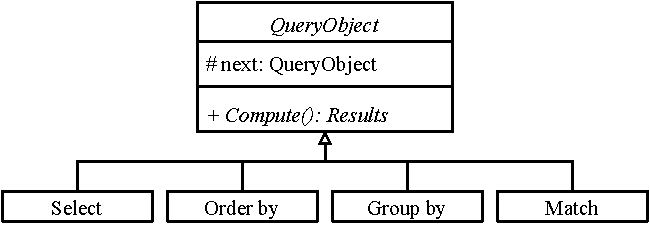
\includegraphics{../img/diaQueryObjects.pdf}\centering
\caption{UML class diagram objektů představující části dotazu.}
\label{figure.diaQueryObjects}
\end{figure}

\clearpage

\begin{figure}[!htp]
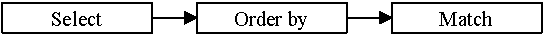
\includegraphics{../img/diaQueryObjectsCon.pdf}\centering
\caption{Propojení objektů pomocí položky \texttt{next} pro dotaz select x match (x) order by x.}
\label{figure.diaQueryObjectsCon}
\end{figure}

\begin{figure}[!htp]
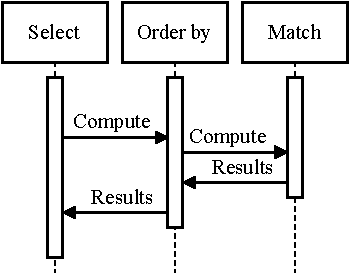
\includegraphics{../img/diaQueryObjectsCall.pdf}\centering
\caption{UML activity diagram rekurzivního volání metody \texttt{Compute} pro dotaz select x match (x) order by x.}
\label{figure.diaQueryObjectsCall}
\end{figure}

\subsection{Paralelizace vykonání dotazu}

Poslední věc nutnou ošetřit je způsob paralelizace dotazu.
Existuje několik možností.
Paralelizace bude provedena pouze interně pro každy objekt nebo dojde k vypracování složitějšího modelu.
V naší představě bychom volili první variantu.
Pomocí ní zaručíme nezávislost objektů a nebudeme nutni vytvářet závislosti mezi objekty.
Při analýze jednotlivých částí budeme vycházet z předpokladu, že existuje \texttt{ThreadPool} vláken.
Do \texttt{ThreadPool} budeme zařazovat úkony k vykonání (\texttt{Tasks}).

\subsection{Formát výsledků} \label{anal.tables}

Mezi částmi dochází k předávání výsledků.
Výsledky musí mít definovaný formát, aby každá část dokázala správně provádět svou logiku.
V části Match dochází ke generování obecných výsledků.
V části Group by dojde k vytvoření skupin a výpočtů agregačních funkcí.
Pokud je v uživatelském dotazu zahrnuto Group by, tak zbylé části musí očekávat jiný formát výsledků.
Daný formát musí obsahovat skupiny a výsledné hodnoty agregačních funkcí.

Obecné výsledky hledání budeme ukládat do tabulky.
Jeden řádek tabulky bude reprezentovat jeden výsledek hledání.
Nyní musíme rozhodnout, jaké informace do tabulky uložíme.
V části Match se pracuje s elementy grafu.
Jeden výsledek hledání obsahuje seznam elementů, které odpovídají vzoru.
Máme dvě možnosti, jak daný výsledek zpracovat.
První varianta v části Match při jeho nalezení vypočte hodnoty všech výrazů obsažených ve zbytku dotazu.
Sloupeček představuje hodnoty jednoho výrazu.
Tato varianta nám nepřišla vhodná, protože by objekt Match musel znát informace o výrazech v celém dotazu.
Navíc výrazy v částech mohou být rozdílné.
Tedy se vytváří nutnost vytvářet sloupečky hodnot v moment, kdy se nepotřebují a tím se navyšuje spotřeba paměti.

\clearpage

Příkladem může být dotaz: 
\begin{code}
select x.P1, ..., x.Pn match (x) -> (y) order by y.P1, ..., y.Pm  
n, m belongs to N and n, m > 1
\end{code}

Zde vidíme množství výrazů.
Pokud bychom aplikovali první variantu, tak v Match části musíme vygenerovat $m + n$ sloupců hodnot.
Z tohoto důvodu chceme zvolit jinou variantu.
Do tabulky budeme ukládat elementy grafu.
Sloupeček tabulky bude reprezentovat jednu proměnnou z dotazu Match.
Tedy tabulka má počet sloupečku rovný počtu unikátních proměnných. 
Pro stejný dotaz vytvoříme pouze dva sloupečky.
Abychom zamezili stejnému problému i z opačné strany (tj. mnoho proměnných a málo výrazů), tak budeme ukládat pouze proměnné, ke kterým se přistupuje v ostatních částech.
Tímto jsme vyřešili paměťový problém, ale nastal problém výkonnosti.
Vyvstává totiž nutnost vypočítávat hodnoty výrazů znova, přestože jsme je už v minulosti počítali (např. při třídění se několikrát porovnává stejný výsledek s jinými).
Problém se dá částečně řešit cachováním výsledků, ale ten ponecháme na analůzu zbylých částí.
V tento moment jsme se rozhodli jít cestou menší paměťové náročnosti na úkor výkonnosti.
Pro výsledky Group by můžeme opět v představě volit tabulku.
Jediný rozdíl bude, že řádek zde bude reprezentovat jednu skupinu (opět uložené elementy grafu) společně s vypočtenými hodnotami agregačních funkcí.

\subsection{Proxy třída jako řádek tabulky}

Musíme být schopni pracovat s řádky tabulek.
Pomocí řádků v tabulce se musí vyhodnotit výrazy v částech Group/Order by a Select.
Vstupním argumentem expression by měl být pouze jeden řádek.
Přesouvání řádku o více sloupcích je drahé.
Pro docílení efektivní práce s řádky budeme řádek reprezentovat proxy třídou.
Proxy třída bude návratová hodnota funkce indexeru tabulky (\texttt{ResultTable[i]}, kde \texttt{i} je index řádku).
Třída poskytne metody pro přístup k elementům nebo výsledkům agr. funkcí ve sloupečcích pro daný řádek tabulky.
V ideálním případě si bude pamatovat pouze index reprezentujícího řádku a odkaz na tabulku.
Nyní pokud budeme chtít vyhodnotit výraz pro $i$-tý řádek tabulky, tak zavoláním indexeru dostaneme proxy třídu a tu použijeme k vyhodnocení výrazu.

\bigskip
\textit{Analyzovali a navrhli jsme obecně způsob vykonání dotazu společně s formátem předávaných výsledků mezi částmi. 
Nyní přejdeme k analýze jednotlivých částí dotazu. 
V analýze jsme se rozhodli vychenat část Select, protože není podstatná pro naši práci.}

\section{Match a prohledávání grafu}

Match část má za úkol najít všechny podgrafy v grafu odpovídající zadanému vzoru.
Vlastnosti hledání jsou definované jazykem PGQL (sekce \ref{req.pgql}).
Vzor se vždy skládá z posloupnosti vrcholů a hran.
Na každý prvek posloupnosti se můžeme dívat jako na placeholder nějakého elementu grafu.

Vlastnosti hledání:
\begin{itemize}

\item Výsledky hledání jsou podgrafy homomorfní se zadaným vzorem.
\item Hrana se může opakovat několikrát v rámci jednoho vzoru.
\item Proměnná hrany ve vzoru se může použít pouze jednou.
\item Dvě rozdílné proměnné mohou obsahovat stejný element.
\item Shodnost elementů se ověřuje pouze na opakující se proměnné.

\end{itemize}

\subsection{BFS vs DFS}

Hledání podgrafu v grafu je obecně složitý problém. 
Cílem této práce není navrhnout algoritmus pro vyhledávání vzoru, proto jsme se rozhodli inspirovat a použít obecný postup k řešení daného problému.
Mezi základní postupy vyhledávání vzoru patří prohledávání do šířky (BFS) a prohledávání do hloubky (DFS) \citep[kap. 4]{graphAlg}. 
Na základě 1. a 2. kapitoly článku \citet{asyncPGX} jsme vybrali algoritmus DFS, jelikož v průběhu prohledávání generuje menší množství mezivýsledů.
To je dáno chováním BFS. 
BFS v každém kroku musí prozkoumat všechny sousedy políček z předešlého kroku.
Toho se docílí vložením nových sousedů do fronty (obecná struktura \texttt{queue} first in first out).
Fronta se tak rychle zvětšuje.
DFS naopak potřebuje znát sousedy pouze aktuálně prohledávaných vrcholů.

\subsection{Hledaný vzor}

K aplikaci algoritmu musíme vytvořit strukturu (vzor) představující hledaný podgraf.
V sekci \ref{anal.mathcandvar} jsme uvedli, že posloupnosti oddělené čárkou budou reprezentovány jako pole tříd obsahující informace o proměnných.
Jedno pole je ekvivalentní jedné posloupnosti.
Pro zřetelnost budeme hovořit o jednom poli jako o řetězci.

Příklad dotazu se dvěma řetězci:
\begin{code}
match (x) -> (y), (x) -> (q)
\end{code}

Řetězce nám nyní budou sloužit k vytvoření vzoru.
Abychom mohli efektivně hledat daný vzor, potřebujeme z řetězců vytvořit souvislé komponenty.
Souvislé komponenty vytvoříme propojením řetězců pomocí opakujících se proměnných.
Tedy dva řetězce jsou propojeny právě tehdy, obsahují-li stejnou proměnnou. 
Propojením všech takových řetězců vytvoříme souvislé komponenty.
Souvislá komponenta představuje hledaný vzor.
Problém vyvstane, pokud nám vzniknou dvě separátní komponenty z jednoho dotazu.
Tento případ nastene právě tehdy, když pro dvě komponenty neexistuje proměnná, která by je propojila.
V takovém případě se můžeme dívat na dotaz, jako na skalární součin výsledků hledání dvou komponent.
Stejný princip aplikujeme, pokud existuje vícero separátních komponent.

Příklad dotazu separátních komponent:
\begin{code}
select x, y match (x), (y)
\end{code}

\subsection{Průběh hledání}

K nalezení všech podgrafů v grafu pořebujeme z každého vrcholu spustit DFS.
Při DFS se bude kontrolovat, jestli průchod odpovídá hledanému vzoru.
Procházení vždy začíná vrcholem, následně přístupem k hranám daného vrcholu a pak koncovému vrcholu hrany. 
K procházení grafu máme navrhnutou strukturu z sekce reprezentace grafu \ref{anal.grafrep}.
Pokud dojde k nalezení podgrafu, tak výsledek bude uložen způsobem z sekce \ref{anal.tables}.

Vyhledávání separátních komponent vyřešíme následovně.
V momentě, kdy nalezneme podgraf odpovídající jedné komponentě, tak se spustí DFS vyhledávání pro komponentu další.
Teprve až projdeme všechny komponenty, výsledek se uloží do tabulky.
V tuto chvíli budeme vlastnit finální výsledek hledáná, který můžeme uložit do tabulky.
Zbavíme se tak nutnosti uchovávat mezivýsledky a následnému tvoření skalárního součinu.

\subsection{Paralelizace hledání}

Nyní přistoupíme k analýze paralelizace hledání.
V paralelním řešení chceme použít co nejmenší počet synchronizačních primitiv.
Ukládání výsledků do společné struktury by způsobilo značny overhead za synchronizaci.
V ideálním případě bude probíhat hledání lokálně, následně pak dojde k efektivnímu mergi.

Jako řešení jsme zvolili jeden ze základních způsobů.
Budeme paralelizovat prohledávání ze startovních vrcholů.
Vyhledávání bude reprezentováno objektem (\texttt{Matcher}).
\texttt{Matcher} vlastní strukturu reprezentující hledaný vzor (\texttt{Pattern}).
Každé vlákno bude vlastnit lokálně svůj \texttt{Matcher}, \texttt{Pattern} a svou tabulku výsledků.
Všechna vlákna budou sdílet thread-safe objekt, který přiděluje části vrcholů grafu (\texttt{VertexDistributor}).
Vlákno vždy zažádá \texttt{VertexDistributor} o určitý počet vrcholů, ze kterých spustí lokálně prohledávání a výsledky uloží do své tabulky.
Nikdy nenastave situace, kdy dva vlákna mají stejný startovní vrchol.
Po vyčerpání všech vrcholů grafu prohledávání končí.
V Single-thread řešení jsou přiděleny všechny vrcholy najednou danému vláknu. 
Rozložení objektů mezi vlákny je zobrazeno na obrázku \ref{figure.diaQueryObjectsMatchPar}. 

\texttt{VertexDistributor} je zde velice důležitý.
Musí rozdělovat malé části vrcholů.
Kdyby rozděloval velké části vrcholů může se stát, že některá vlákna budou mít mnohem více práce.
Je to protože reálné grafy nemají obecně rovnoměrné rozložení hran.
Jedno vlákno by mohlo dostat vrholy nacházející se v oblasti s množstvím hran, zatímco jiné vlákno by procházelo řídkou oblastí.
Jelikož se rychle vyčerpaly startovní vrcholy, tak vlákno z řídké oblasti ukončí svou práci mnohem dříve něž vlákno první.
Nyní se musí čekat na dokončení práce prvního vlákna.

\subsection{Merge výsledků hledání}

Po dokončení hledání je nutno vyřešit mergování výsledků jednotlivých vláken.
Kdybychom ponechali výsledky bez úpravy, tak nedokážeme rovnoměrně rozdělit práci mezi vlákna v paralelních řešeních Order/Group by.
Cílem je vytvořit jednu tabulku obsahující všechny výsledky.
K vyhnutí překopírovávání všech výsledků vláken využijeme následující princip.
Sloupeček tabulky bude tvořen polem polí fixní délky.
V jazyce C\# \texttt{List<Element[FixedArraySize]>}.
V kroku mergování nyní pouze překopírujeme odkazy na pole místo samotných výsledků.
Avšak, pořád nám zůstává nutnost překopírovat výsledky posledních polí sloupečků, která jsou nezaplněná.
Volbou vhodné hodnoty \texttt{FixedArraySize} se bude překopírovávat pouze malé množství výsledků.
Konkrétní volba hodnoty je heuristická a vyplývá z vlastností grafu a počtu nalezených výsledků.
Pro naše učely během implementace zkusíme zvolit prvně $n/\log_2 n$ ($n = $ \#výsledků hledání) pro single-thread a pro paralelní zpracování $(n/\log_2 n)/\#threads$.
$log_2 n$ odpovídá počtu přealokování při plnění dynamického pole $n$ položkami.
Mergování bude probíhat opět paralelně.
Nabízí se dva způsoby.
Vlákno merguje pouze jeden sloupeček nebo dojde k dvoucestnému mergi výsledků vláken.
Nyní je obtížné odhadnou správné řešení a proto jej ponecháme na dobu implementace.    

\begin{figure}[!htp]
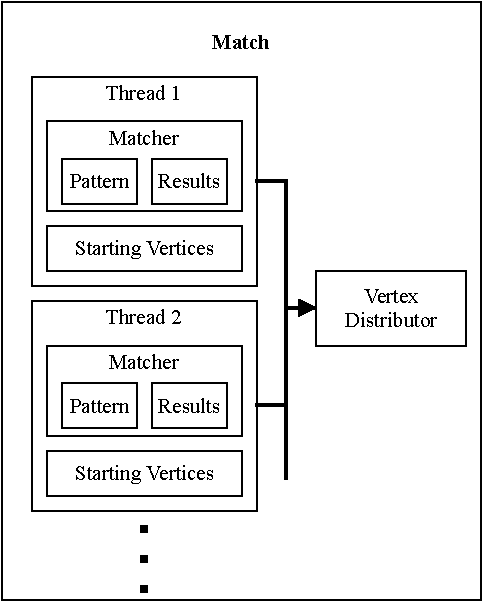
\includegraphics{../img/diaQueryObjectsMatchPar.pdf}\centering
\caption{Diagram paralelizace prohledávání grafu.}
\label{figure.diaQueryObjectsMatchPar}
\end{figure}

\bigskip
\textit{Zbývá nám analyzovat a navrhnout Group by a Order by.
Je nutné si uvědomit potřebu analýzy daných částí.
Analýza nám pomůže pochopit jejich fungování, což nám umožní je lépe porovnat s vylepšenými řešeními. 
Zároveň také tvoří odrazový můstek pro návrh vylepšených řešení.}

\section{Order by}

Order by si klade za cíl setřídit vyhledané výsledky z části Match pomocí zadaných klíčů.
Pořadí klíčů určuje pořadí porovnání.
Výsledky se porovnávají zleva doprava.
To znamená, pokud jsou dva klíče stejné, postoupí se k porovnání s klíčem dalším.
Rovnost dvou výsledků nastává právě tehdy, když mají stejné hodnoty pro všechny klíče. 
Pro klíč se také definuje, jestli má třídění probíhat v rostoucím nebo klesajícím pořadí.
Defaultní pořadí je chápáno jako rostoucí. 
Potřebujeme určit, jakým způsobem budou výsledky hledání setříděny.
Musíme vybrat algoritmus a následně navrhnout způsob efektivního třídění tabulky výsledků.

\subsection{Výběr algoritmů a paralelizace}

Existuje mnoho algoritmů pro třídění.
Chtěli bychom zvolit již prozkoumané a zároveň běžně používané třídící algoritmy.
Mezi náš výběr padli Merge sort nebo Quick sort.
Jsou ideální volba, protože pro ně již existuje paralelní verze.
Při implementaci chceme ideálně použít již existující knihovny nebo implementace. 

\subsection{Quick sort vs Merge sort}

Uvedeme krátké porovnání na základě 3. kapitoly průvodce algoritmů \citep{labyrint}. 
Merge sort má časovou složitost $ \Theta(n\log n) $ i v nejhorším případě, zatímco Quick sort stejné složitosti dociluje pouze v průměrném případě.
V nejhorším případě má $\Theta(n^2)$.
Merge sort potřebuje $\Theta(n)$ pomocné paměti a je to stabilní třídící algoritmus.
Quick sort pouze $\Theta(\log n)$, ale nejedná se stabilní třídění.
K implementaci stabilního Quick sortu je potřeba $\Theta(n)$ pomocné paměti.
Quick sort značně závisí na výběru pivota.
V našem případě bude obtížné ho volit správně, protože nedokážeme říci nic o rozložení tříděných dat.
Z tohoto důvodu bychom volili raději Merge sort.  

\subsection{Třídění pomocí indexů}

Hlavním problémem Order by je třídění tabulky výsledků.
V sekci \ref{anal.tables} jsme definovali formát výsledků a navrhli proxy třídy pro výpočet výrazů.
Setřídit tabulku v našem smyslu znamená setřídit řádky pomocí klíčů zadaných uživatelem.
Pro zjištění shodnosti dvou řádků musíme vypočítat hodnoty jejich klíčů pomocí výrazů a následně je porovnat.
Přesouvání řádků v tabulce, která má více než jeden sloupec, by představovalo značné zpomalení.
Uvedli jsme, že výrazy pro řádky dostanou na vstupu proxy třídu řádků.
Proxy třída se v naší představě získá voláním funkce indexeru na tabulce výsledků.
Daný princip nám umožní vytvořit pole indexů v rozsahu počtu řádek tabulky.
Indexy budou setříděny namísto pravých řádků vybraným algoritmem a při porovnání dojde k získání proxy tříd a výpočtu výrazů.
Přistup nám umožní vyřadit přesouvání řádků, ale zase potřebujeme lineární pamět na pole indexů.
Po dokončení třídění se pole použije jako indexační struktura.

\subsection{Optimalizace porovnání Property hodnot} \label{anal.order.opt1}

Třídění obvykle představuje opakované porovnání jednoho prvku s ostatními v řadě za sebou.
Pro pokaždé takové porovnání v řadě počítáme stejnou hodnotu výrazu opakovaně.
Porovnání pomocí \texttt{ID} pouze přistupuje k položce elementu grafu.
Problém nastane, když budeme porovnávat pomocí Property.
V takovém případě musíme přistoupit k tabulce \texttt{elType} (sekce \ref{anal.grafrep}), zjistit existenci přistupované Property a následně přistoupit k její hodnotě.
Danou situaci můžeme vyřešit částečně cachování výsledků výrazů.
Budeme si pamatovat poslední porovnané řádky a jejich hodnoty.
Pokud dojde k porovnání řádků pro který byl výraz již vypočítán, tak použijeme zachovanou hodnotu.

\subsection{Optimalizace porovnání stejných elementů}

Dalši možná optimalizace porovnání může nastat v případě, pokud pro dotaz nad grafem platí \#Vrcholů $<<$ \#Hran.
Daná vlastnost může mít za následek, že porovnávané řádky budou obsahovat často obsahovat stejné elementy pro dotazy typu:
\begin{code}
select x.PropOne match (x) -> (y) order by x.PropOne;
\end{code}
V takovém dotazu by hledání mělo vygenerovat několik výsledků se stejným elementem v proměnné x.
Počet takových výsledků zde odpovídá počtu hran vrcholů x.
Abychom předešli opakovanému porovnávání hodnot Property stejných elementů, tak než přistoupíme k výpočtu výrazů porovnáme \texttt{ID} přistupovaných elementů.
Tedy využijeme dvou optimalizací.
Budeme si cachovat poslední výsledky výrazů a navíc omezíme porovnání výsledků se stejnými elementy.

\subsection{Optimalizace v paralelním prostření}

Vymysleli jsme optimalizace porovnání.
Doteď jsme však předpokládali, že porovnání probíhá v jednom vlákně.
Druhá optimalizace funguje i v paralelním prostřední, protože se jedná pouze o čtení statických hodnot.
Avšak první optimalizace vytváří problém.
V prvním případě dochází k uchovávání výsledků lokálních pro vlákno a existence sdíleného úložiště by vytvořilo race condition.
Vlákna by se snažila číst a ukládat výsledky ze sdíleného úložiště a docházelo by k nedefinovanému chování.
Problém se dá vyřešit například tak, že každé vlákno bude vlastnit svoje objekty s cachí výsledků.
V průběhu implementace budeme muset najít vhodnou techniku ukládání, aby došlo ke zrychlení třídění.

\section{Group by}

Group by seskupuje výsledky hledání podle uživatelem zadaných klíčů.
Dva výslekdy patří do stejné skupiny právě tehdy, když se shodují ve všech hodnotách klíčů.
Musíme být schopni vypočítat agregační funkce pro skupiny.
K tomu již máme navržené způsoby z sekce Expressions (\ref{anal.expressions}).
Zbývá nám vymyslet způsob ukládání mezivýsledku a algoritmy k vykonání.

\subsection{Módy Group by}

Group by představuje dle našeho pohledu dva módy vykonání.
První mód obsahuje v dotazu část Group by a libovolné množství agregačních funkcí.
Dojde k vytvoření skupin a výpočtu výsledků funkcí pro každou skupinu.
Tento mód budeme označovat \textbf{Group by}.
Druhý mód nemá v dotazu část Group by, ale pouze agregační funkce v ostatních částech.
Zde automaticky dochází k předpokladu, že všechny výsledky patří do stejné skupiny.
Tedy je vytvořena pouze jedna skupina a pro ni se vypočtou hodnoty agregačních funkcí.
Mód nazveme \textbf{Single group Group by}.


\subsection{Úložiště mezivýsledků agregačních funkcí}

V sekci Expressions (\ref{anal.expressions}) jsme navrhli objekt, který obsahuje logiku výpočtu funkce a na vstupu dostává úložiště výsledku.
Očekává se, že pro každou skupinu bude existovat úložiště.
Úložiště musí obsahovat prostor pro výsledky všech počítaných funkcí.
Vymysleli jsme dva způsoby:

\begin{itemize}

\item \textbf{Bucket} - každá skupina bude vlastnit pole objektů. 
Pole bude mít délku rovnou počtu počítaných agregačních funkcí.
Objekty představují úložiště výsledků funkcí.

\item \textbf{List} - výsledky všech skupin jsou uchovávány v dvoudimenzionálním poli, tj. primitivní tabulce.
Sloupeček představuje výsledky jedné agregační funkce.
Jedné skupině pak přináleží řádek.
Každé skipině bude přidělen index řádku.
Nyní pokud budeme chtít výsledky funkcí skipiny, stačí přistoupit skrze přidělený index ke chtěnému výsledku.
\end{itemize}

Následuje ukázka možné implementace v jazyce C\#:
\begin{code}
Bucket:
BucketResult[] groupAggFuncResults; 
class BucketResult {}
class BucketResult<T>: BucketResult { T value; }

List:
ListResults groupsAggFuncResults;
// are accessed via tableIndex.
class ListResults { ListHolder[] holders; }
class ListHolder {}
class ListHolder<T> : ListHolder { List<T> values }
\end{code}

První způsob je náročnější na paměť oproti druhému způsobu, neboť je zde nutnost vytvářet objekty a pole pro každou skipinu.
Avšak, v druhém způsobu jsme nuceni přistupovat k výsledkům pomocí indirekce.
Výhoda Bucket spočívá v jeho jednoduchém přemisťování (chápeme-li pole jako referenci) a izolaci od ostatních výsledků skupin.
V takovém případě jsme schopni přesouvat výsledky skupiny aniž bychom museli kopírovat jejich hodnoty.
Předpokládáme, že bucket bude výhodnější pro paralelní zpracování díky izolaci od ostatních výsledků, jelikož počet skupin není dopředu znám.
V List budeme muset dynamicky rozšiřovat pole.
Při rozšíření nastane race condition, který budeme muset ošetřit.

\subsection{Single thread zpracování}

Po celou dobude budeme pracovat s tabulkou výsledků Match části.
Pro vykonání Group by se nám nabízí několik možností.
První možnost je řádky tabulky setřídit a následně při iteraci výtvářet skupiny a počítat agregační funkce.
Myslíme, že možnost přináší zbytečný overhead za porovnání při třídění, protože pro každé porovnání musíme vypočítat hodnotu výrazu.
Z tohoto důvodu chceme využít strukturu, která bude interně použivát hashovací tabulku (mapa/slovník).
Záznam v tabulce bude dvojice \texttt{key/value}. 
\texttt{key} je zde index do tabulky výsledků z Match části (nikoliv proxy třída).
Chceme ukládat pouze index abychom ušetřili paměť za pointr na tabulku.
Porovnání vyvolá získání proxy třídy a následné evaluaci hodnot výrazů.
\texttt{value} obsahuje strukturu pro výsledky agregačních funkcí.
Pro Bucket to bude pole objektů a pro List to bude index do tabulky výsledků agregačních funkcí.
Pro výsledek bude vypočítáná hash na základě hodnot klíču a vložena do hashovací tabulky.
Pokud už je obsažen v tabulce, tak se pouze pro získanou \texttt{value} (pole nebo index) aktualizují hodnoty výsledků agregačních funkcí.
V opačném případě bude vložen nový záznam s novou \texttt{value}.
Pro Single group Group by stačí pouze iterovat skrze tabulku a počítat agregační funkce.

\subsection{Optimalizace při výpočtu hash hodnoty}

Minulý přístup nám nabízí jednu optimalizaci k ušetření opakovaného výpočtu hodnoty výrazu klíčů.
Hashovací tabulka při vložení dvojice v prvním kroku vypočte hodnoty klíčů a vypočte jejich hash.
Výsledek se vloží do patřičné přihrádky.
Pokud nastala kolize, tak se prvky musí porovnat.
Při tomto porovnání se opět musí vypočíst hodnoty výrazů vkládané dvojice.
Zde mužeme využít chvíle výpočtu hash hodnoty.
Budeme cachovat hodnoty výrazů a následně je znovu použít při porovnání.
Nicméně, pravděpodobně budeme nutni vytvořit závislost mezi objektem počítajícím hash hodnotu a objektem provádějícím porovnání.
Stejný princip jsme použili při optimalizaci porovnání v sekci \ref{anal.order.opt1}.
Nastávají pro něj stejné problémy v paralelním prostředí.

\subsection{Paralelní zpracování}


\subsection{Global Group by}


\subsection{Two-step Group by}

\subsection{Local + 2-way merge Group by}

\subsection{Paralelizace Single group Group by}


\section{Návrh vylepšení}
\label{anal.improvement}